  \begin{figure}[H]
  \begin{center}
  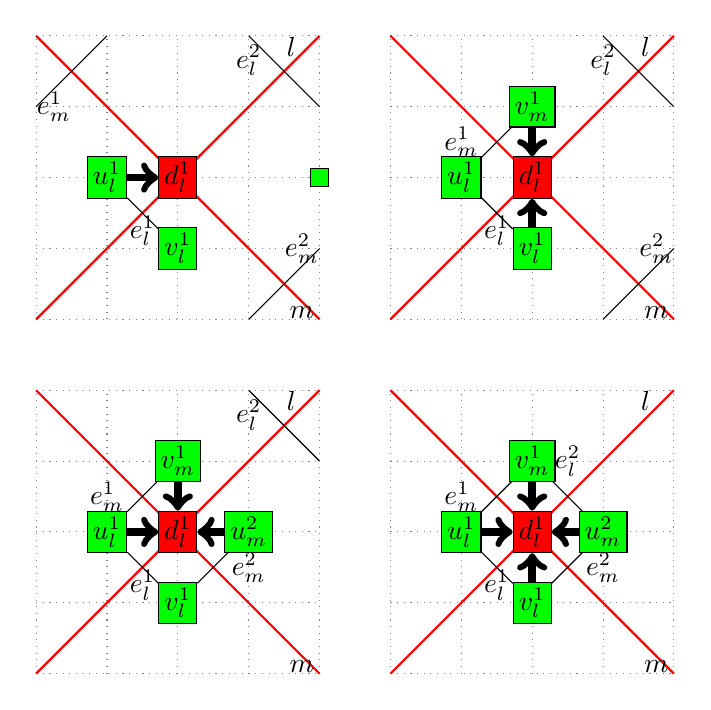
\begin{tikzpicture}[scale=0.45]
    \draw[color=gray, style=dotted] (0,0)  
      grid[xstep=2cm, ystep=2cm] (8cm,8cm);
  	\node(u1l) at (2,4) [draw,fill=green,inner sep=2pt] {$u^1_l$};
  	\node(v1l) at (4,2) [draw,fill=green,inner sep=2pt] {$v^1_l$};
    \node at (8,4) [draw,fill=green] {};
	\draw[red,thick] (0,0) -- (8,8); 
	\draw[red,thick] (0,8) -- (8,0); 
    \node(d1l) at (4,4) [draw,fill=red,inner sep=2pt] {$d_l^1$};
    \node at (7.2,7.7) [draw=none] {$l$};
    \node at (7.5,0.2) [draw=none] {$m$};
    \node at (3,2.5) [draw=none] {$e_l^1$};
    \draw (0,6) -- (2,8);
    \node at (0.5,6) [draw=none] {$e_m^1$};
    \draw (6,0) -- (8,2); 
    \node at (7.5,2) [draw=none] {$e_m^2$};
    \draw(u1l) to (v1l);
    %\draw[color=black, style=dashed] (v1l) edge[line width=2.7pt,->] (d1l);    
    \draw[color=black] (u1l) edge[line width=2.7pt,->] (d1l);
    \draw (6,8) -- (8,6);
    \node at (6,7.3) [draw=none] {$e_l^2$};
    
    
  \begin{scope}[shift={(10,0)}]
    \draw[color=gray, style=dotted] (0,0)  
      grid[xstep=2cm, ystep=2cm] (8cm,8cm);
  	\node(u1l) at (2,4) [draw,fill=green,inner sep=2pt] {$u^1_l$};
  	\node(v1l) at (4,2) [draw,fill=green,inner sep=2pt] {$v^1_l$};  	
    \node(v1m) at (4,6) [draw,fill=green,inner sep=2pt] {$v^1_m$};
	\draw[red,thick] (0,0) -- (8,8); 
	\draw[red,thick] (0,8) -- (8,0); 
    \node(d1l) at (4,4) [draw,fill=red,inner sep=2pt] {$d_l^1$};
    \node at (7.2,7.7) [draw=none] {$l$};
    \node at (7.5,0.2) [draw=none] {$m$};
    \node at (3,2.5) [draw=none] {$e_l^1$};
    \draw (u1l) -- (v1m);
    \node at (2,5) [draw=none] {$e_m^1$};
    \draw (6,0) -- (8,2); 
    \node at (7.5,2) [draw=none] {$e_m^2$};
    \draw(u1l) to (v1l);
    \draw[color=black] (v1m) edge[line width=2.7pt,->] (d1l);    
    \draw[color=black] (v1l) edge[line width=2.7pt,->] (d1l);  
    \draw (6,8) -- (8,6);
    \node at (6,7.3) [draw=none] {$e_l^2$};
  \end{scope}
  
    \begin{scope}[shift={(0,-10)}]
    \draw[color=gray, style=dotted] (0,0)  
      grid[xstep=2cm, ystep=2cm] (8cm,8cm);
  	\node(u1l) at (2,4) [draw,fill=green,inner sep=2pt] {$u^1_l$};
  	\node(v1l) at (4,2) [draw,fill=green,inner sep=2pt] {$v^1_l$};  	
    \node(v1m) at (4,6) [draw,fill=green,inner sep=2pt] {$v^1_m$};    
    \node(u2m) at (6,4) [draw,fill=green,inner sep=2pt] {$u^2_m$};
	\draw[red,thick] (0,0) -- (8,8); 
	\draw[red,thick] (0,8) -- (8,0); 
    \node(d1l) at (4,4) [draw,fill=red,inner sep=2pt] {$d_l^1$};
    \node at (7.2,7.7) [draw=none] {$l$};
    \node at (7.5,0.2) [draw=none] {$m$};
    \node at (3,2.5) [draw=none] {$e_l^1$};
    \draw (u1l) -- (v1m);
    \node at (2,5) [draw=none] {$e_m^1$};
    \draw (v1l) -- (u2m); 
    \node at (6,3) [draw=none] {$e_m^2$};
    \draw(u1l) to (v1l);
    \draw[color=black] (u1l) edge[line width=2.7pt,->] (d1l);    
    \draw[color=black] (v1m) edge[line width=2.7pt,->] (d1l); 
    \draw[color=black] (u2m) edge[line width=2.7pt,->] (d1l);  
    \draw (6,8) -- (8,6);
    \node at (6,7.3) [draw=none] {$e_l^2$};
  \end{scope}
  
      \begin{scope}[shift={(10,-10)}]
    \draw[color=gray, style=dotted] (0,0)  
      grid[xstep=2cm, ystep=2cm] (8cm,8cm);
  	\node(u1l) at (2,4) [draw,fill=green,inner sep=2pt] {$u^1_l$};
  	\node(v1l) at (4,2) [draw,fill=green,inner sep=2pt] {$v^1_l$};  	
    \node(v1m) at (4,6) [draw,fill=green,inner sep=2pt] {$v^1_m$};    
    \node(u2m) at (6,4) [draw,fill=green,inner sep=2pt] {$u^2_m$};
	\draw[red,thick] (0,0) -- (8,8); 
	\draw[red,thick] (0,8) -- (8,0); 
    \node(d1l) at (4,4) [draw,fill=red,inner sep=2pt] {$d_l^1$};
    \node at (7.2,7.7) [draw=none] {$l$};
    \node at (7.5,0.2) [draw=none] {$m$};
    \node at (3,2.5) [draw=none] {$e_l^1$};
    \node at (5,6) [draw=none] {$e_l^2$};
    \draw (u1l) -- (v1m);
    \node at (2,5) [draw=none] {$e_m^1$};
    \draw (v1l) -- (u2m); 
    \node at (6,3) [draw=none] {$e_m^2$};
    \draw(u1l) to (v1l);
    \draw(v1m) to (u2m);
    \draw[color=black] (u1l) edge[line width=2.7pt,->] (d1l);    
    \draw[color=black] (v1m) edge[line width=2.7pt,->] (d1l); 
    \draw[color=black] (u2m) edge[line width=2.7pt,->] (d1l);  
    \draw[color=black] (v1l) edge[line width=2.7pt,->] (d1l);  
  \end{scope}
  
  
  \end{tikzpicture}
  \caption{Two gap lines $l$ and $m$ intersecting at a point $d^1_l$. Four figures relate to four cases in the proof. The top left is related to Case 1, the top right to Case 2, the bottom left to Case 3 and the bottom right to Case 4.}
  \label{key_lemma_two_gaps}
  \end{center}
  \end{figure}
